\section*{User Walkthrough 3}

User Walkthrough 3 shows \p{1} releasing an update to \g{1}, \g{2}, and \p{2} downloading it. If User Walkthrough 2 is valid then we will be able to successfully download \g{2} as we did with \g{1}.

\begin{enumerate}[itemsep=2.5pt]

  \item \textbf{\p{1} is the original uploader of \g{1} and \p{2} has already purchased \g{1}.}

  Given from User Walkthrough 1

  \item \textbf{\p{1} uploads an update to \g{1}, \g{2}.}

  \small Transaction hash = 0x0ea6739a1b93add5135e02db3e6030103582ed1cf4240c00ed2e05cfad943a80\normalsize

  \item \textbf{\p{2} will hit the `check for updates' button and see \g{2} in their library.}
  
  The screenshot showing the updated library screen with the new version of the game and logs showing \p{2} querying the blockchain for the new update.


  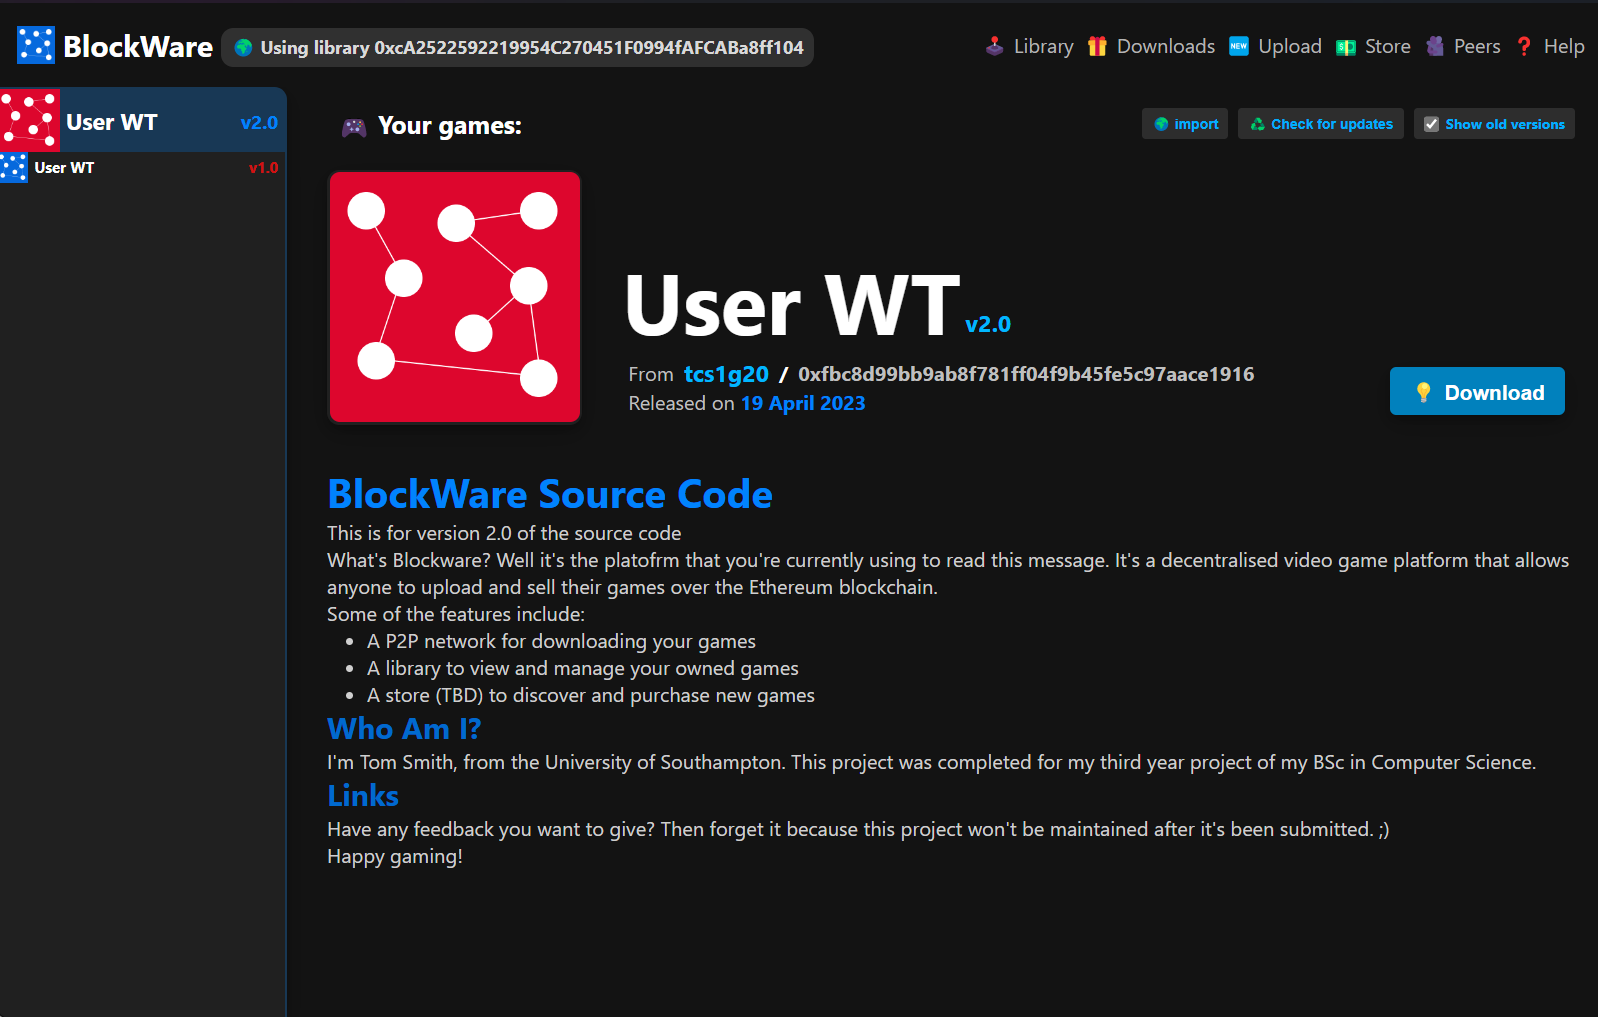
\includegraphics[width=.45\textwidth]{assets/images/user-walkthrough/3/new-library.png}

\begin{lstlisting}[breaklines=true, postbreak=\mbox{\textcolor{red}{$\hookrightarrow$}\space}]
2023-04-19T14:39:14.424+0100	[DEBUG]	library/library.go:291	Checking for game updates
2023-04-19T14:39:14.915+0100	[INFO]	library/library.go:303	Found 1 updates
2023-04-19T14:39:14.915+0100	[DEBUG]	library/library.go:307	1 game updates added successfully
\end{lstlisting}
  

\end{enumerate}